% Results. The earlier combined Results and Discussion draft remains available
% in results_discussion_draft.tex for comparison.

The three monitoring conditions defined in \Cref{subsec:experimental_design} differed in when, or whether, new MLCW observations became available for model updating. The results first describe monthly estimation while finalized MLCW records were temporarily unavailable. They then examine less frequent field measurements and the absence of subsequent MLCW measurements.

\subsection{Monthly estimation during delayed MLCW data delivery}
\label{subsec:results_delayed_delivery}

The estimation and update design comprised 23 complete six-month cycles from 05/2013 to 10/2024 (\Cref{fig:results_delayed_cycles}). After each cycle, the newly finalized MLCW observations expanded the calibration record used for the next cycle. Each cycle produced six monthly estimates for each of the six depth sections, resulting in 138 estimates per section.

\begin{figure}[htbp]
  \centering
  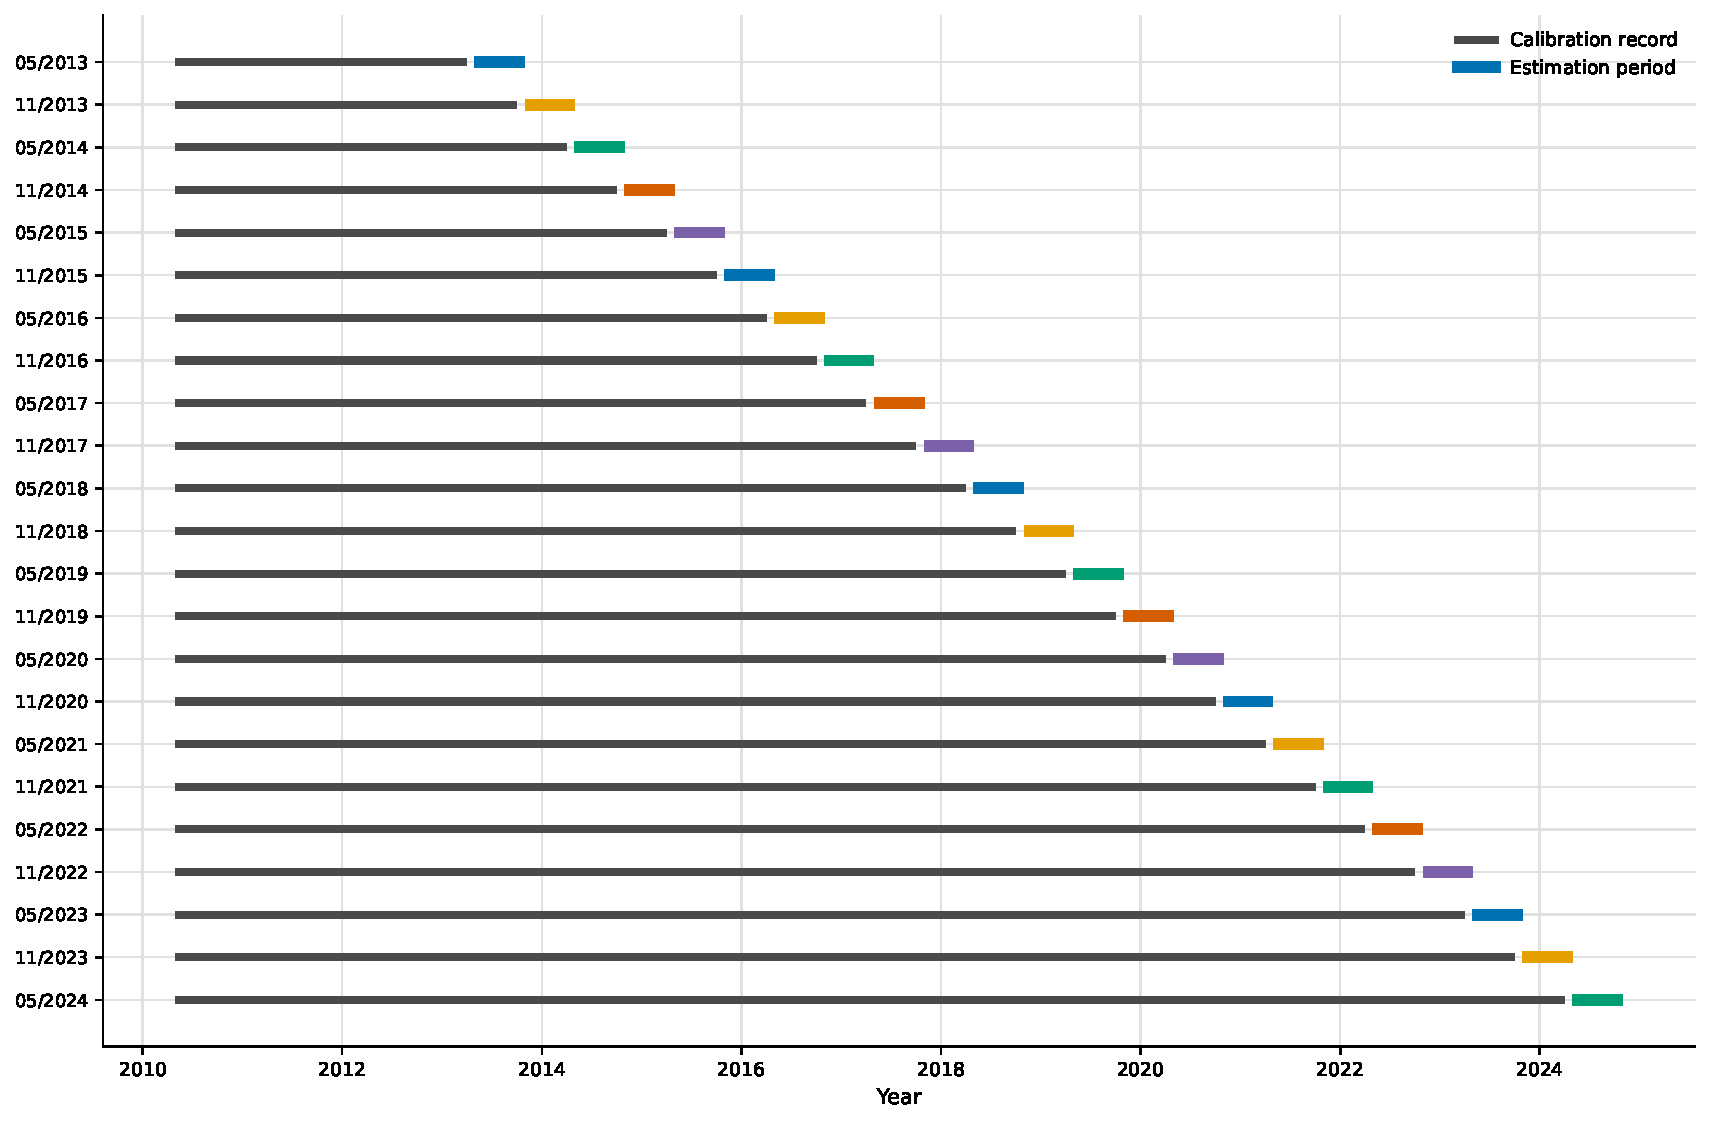
\includegraphics[width=0.98\textwidth]{figures/fig_results_delayed_cycle_timeline.pdf}
  \caption[Calibration and estimation periods during delayed MLCW data delivery.]{Successive calibration and estimation periods used to evaluate monthly deformation increments while finalized MLCW records were unavailable. The five colors repeat to distinguish adjacent estimation periods and do not represent different experimental conditions.}
  \label{fig:results_delayed_cycles}
\end{figure}

The observed and estimated monthly increments followed similar temporal patterns in the upper four sections, whereas larger differences occurred in S5 and S6 (\Cref{fig:results_delayed_monthly_estimates}). This depth-dependent contrast was also evident in \Cref{fig:results_delayed_scatter}, where the estimates for S1--S4 remained closer to the line of exact agreement than those for the two deepest sections.

\begin{figure}[p]
  \centering
  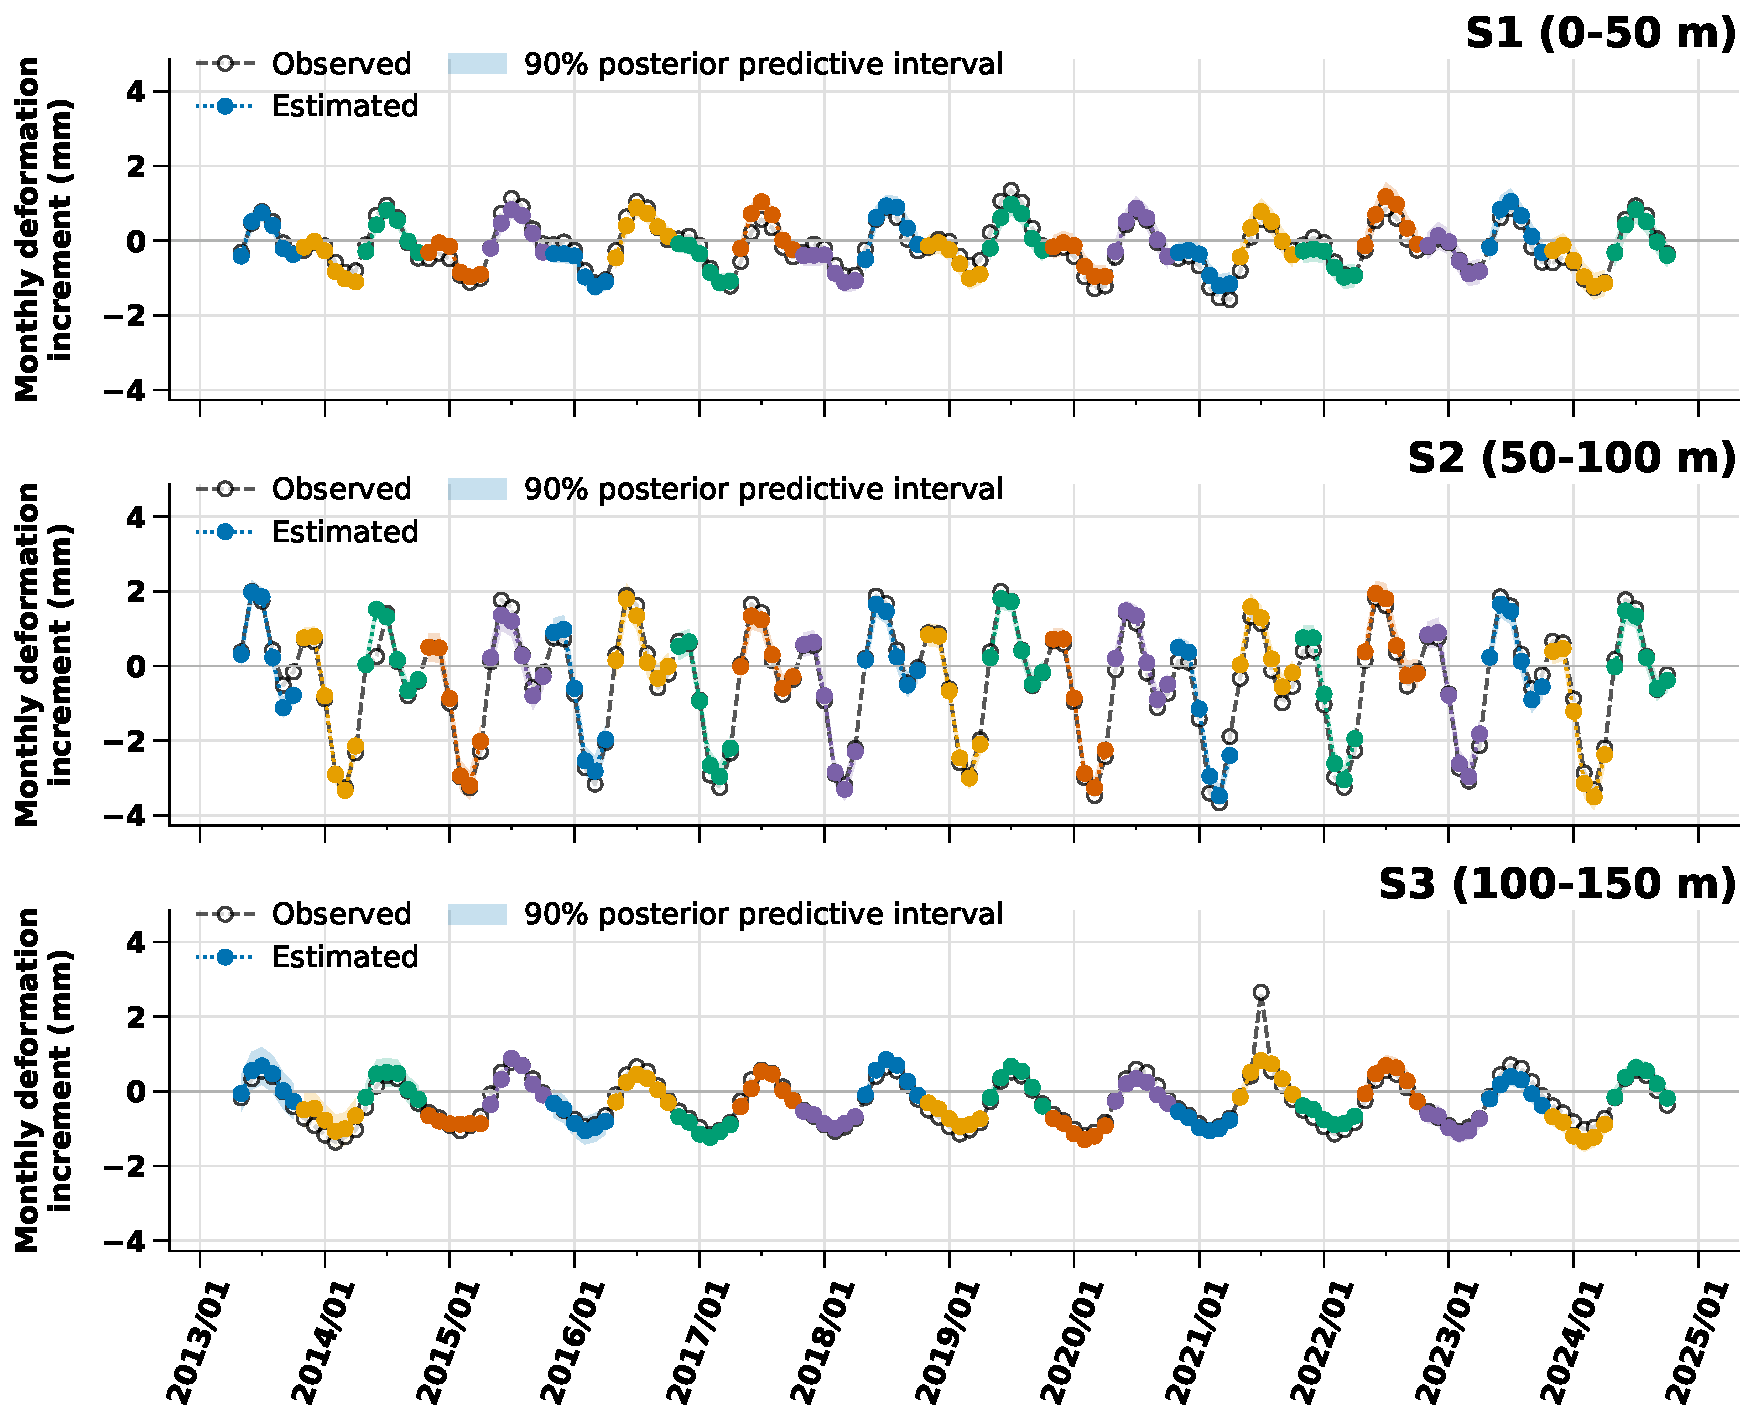
\includegraphics[width=0.98\textwidth]{figures/fig_results_delayed_monthly_estimates_s1_s3.pdf}
  \caption[Observed and estimated monthly deformation increments by depth section.]{Observed and estimated monthly deformation increments for S1--S3. The black lines show observations, colored dotted lines show estimates, and shaded bands show the 90\% Bayesian posterior predictive intervals. The five colors repeat across successive estimation periods.}
  \label{fig:results_delayed_monthly_estimates}
\end{figure}

\begin{figure}[p]
  \ContinuedFloat
  \centering
  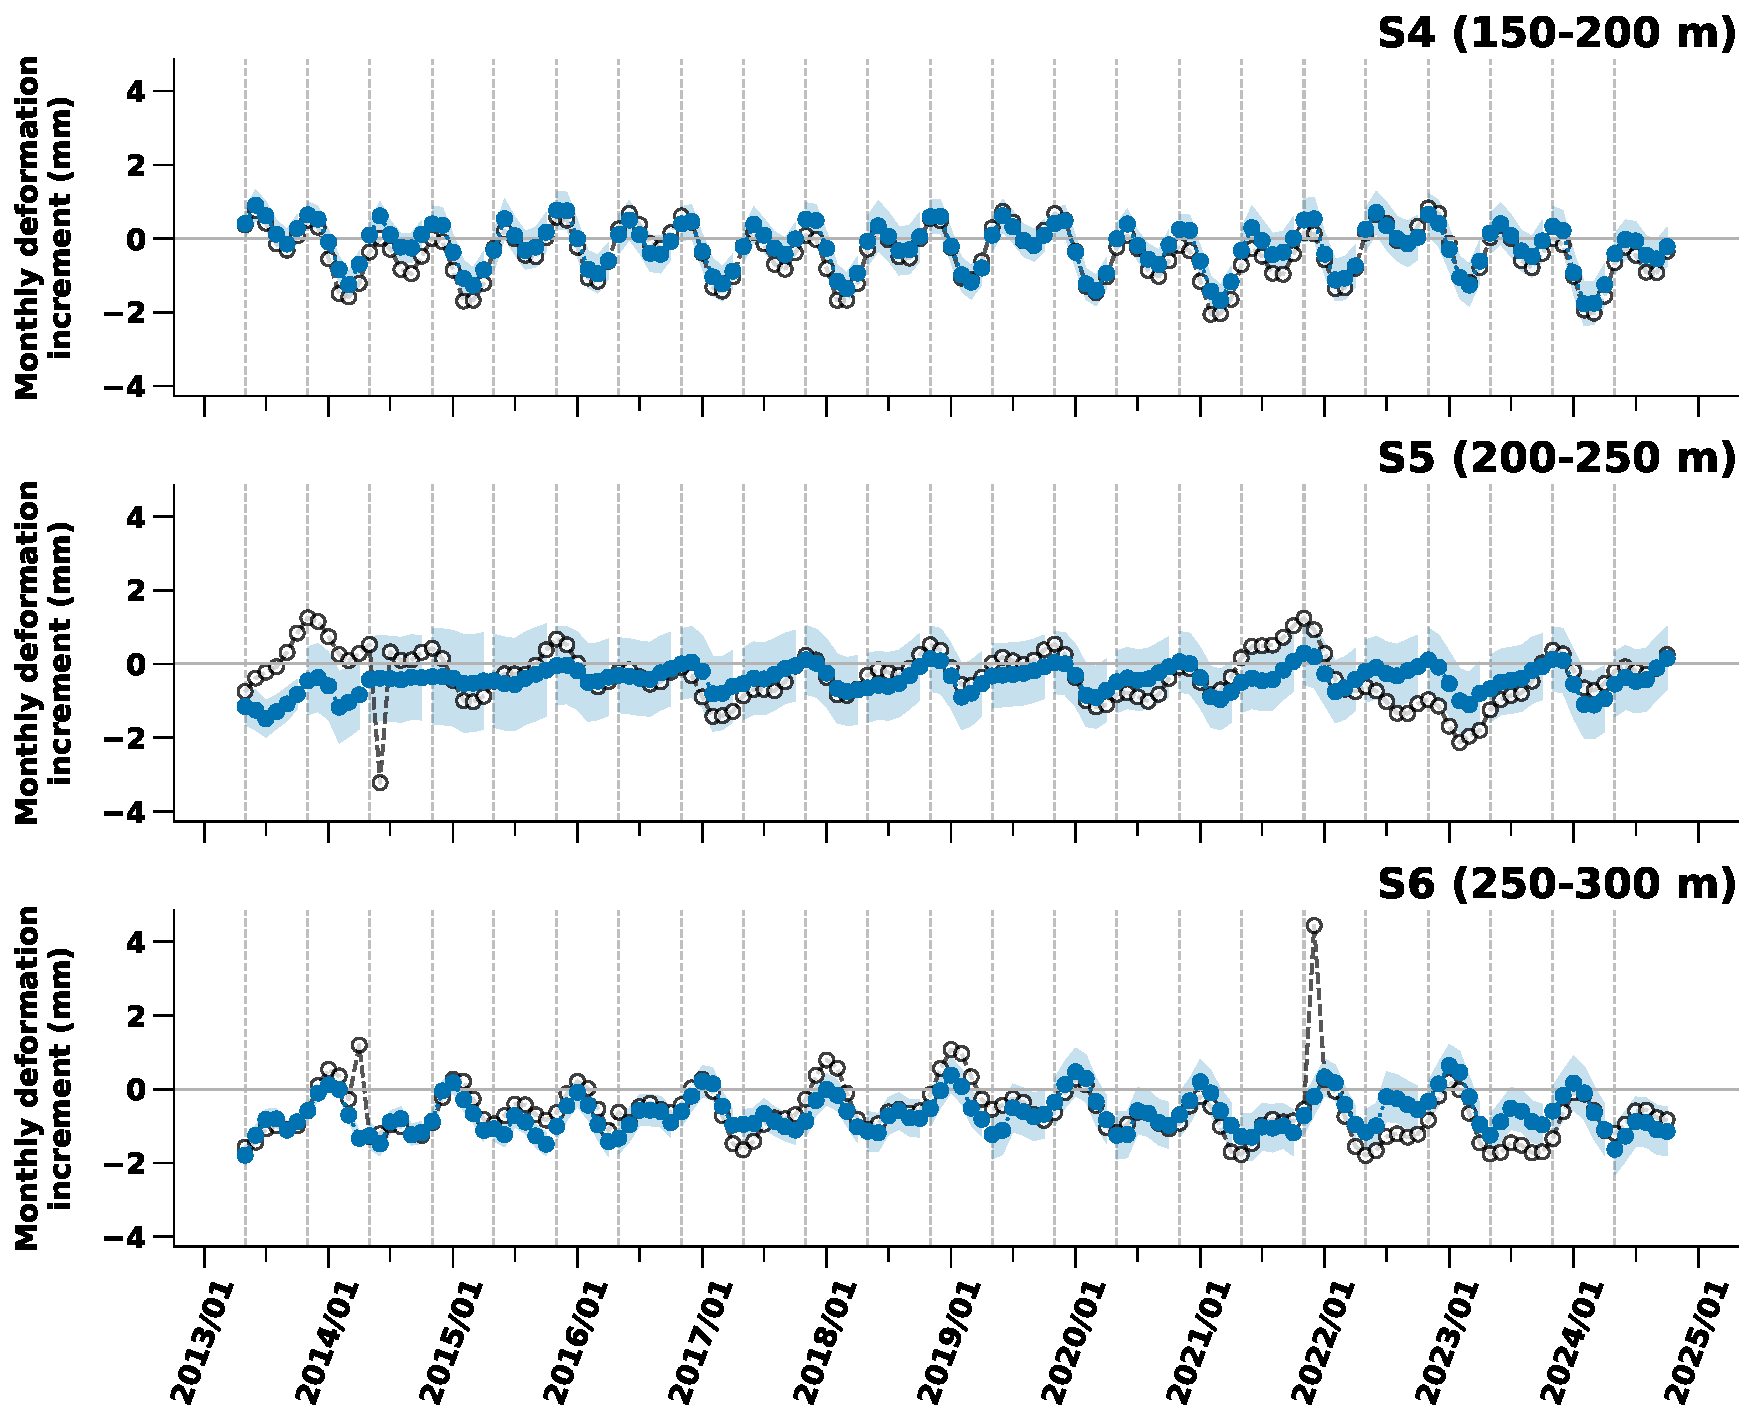
\includegraphics[width=0.98\textwidth]{figures/fig_results_delayed_monthly_estimates_s4_s6.pdf}
  \caption[]{Observed and estimated monthly deformation increments for S4--S6, continued from the preceding page.}
\end{figure}

\begin{figure}[p]
  \centering
  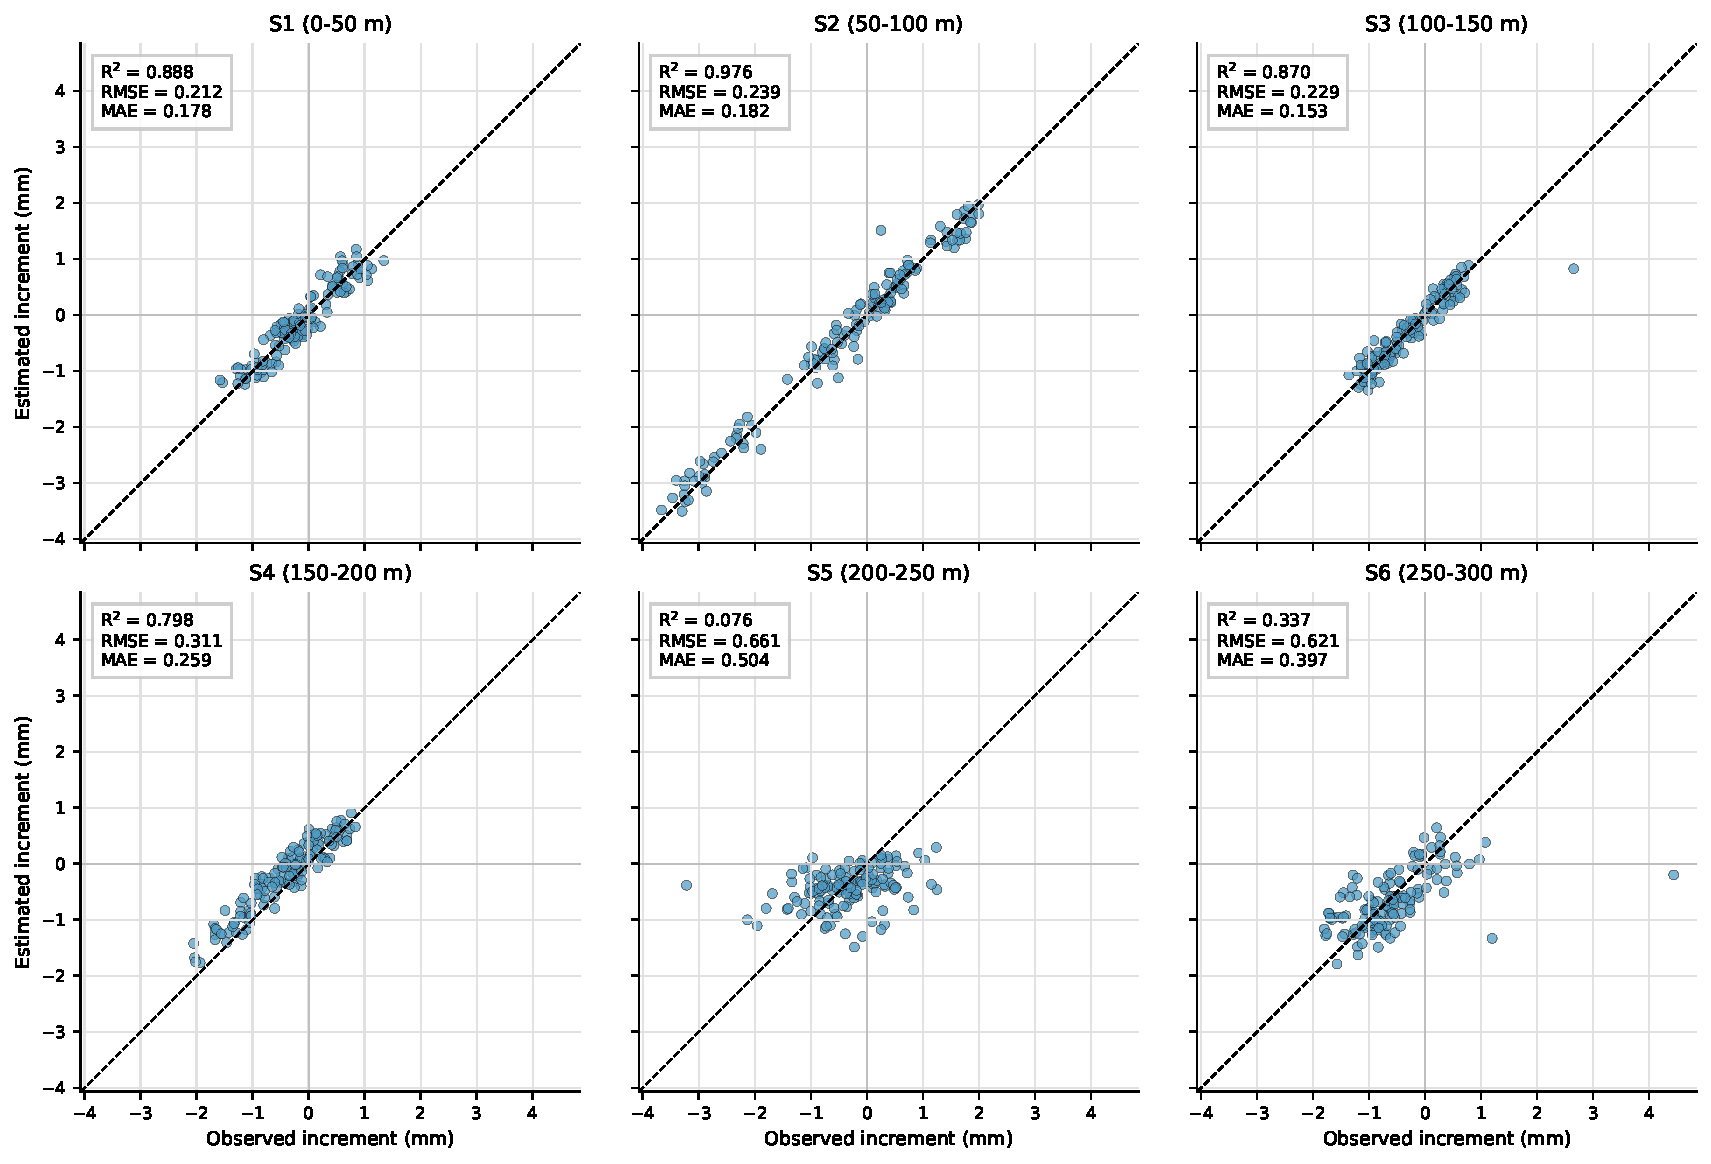
\includegraphics[width=0.98\textwidth]{figures/fig_results_delayed_prediction_vs_observed.pdf}
  \caption[Estimated versus observed monthly deformation increments.]{Estimated versus observed monthly deformation increments for the six depth sections. The dashed line represents exact agreement. RMSE and MAE are reported in mm/month.}
  \label{fig:results_delayed_scatter}
\end{figure}

\FloatBarrier

Point-estimate performance confirmed the differences among depth sections (\Cref{tab:delayed_performance_interval}). Across all sections, the model reached $R^2=0.778$, RMSE~$=0.423$~mm/month, and MAE~$=0.279$~mm/month. Section-level $R^2$ ranged from 0.076 at S5 to 0.976 at S2. RMSE ranged from 0.212~mm/month at S1 to 0.661~mm/month at S5, while MAE ranged from 0.153~mm/month at S3 to 0.504~mm/month at S5. Among the six sections, S5 therefore had both the lowest $R^2$ and the largest RMSE and MAE.

The posterior predictive intervals provided a separate measure of model performance. The nominal 90\% intervals achieved a pooled empirical coverage of 78.019\% and a mean width of 0.904~mm/month. The empirical coverage therefore remained below the nominal level. Coverage ranged from 65.942\% at S6 to 88.406\% at S2, while S5 had the widest mean interval at 1.848~mm/month. Point error, interval width, and empirical coverage therefore did not rank the six sections in the same order.

\begin{table}[htbp]
  \centering
  \small
  \renewcommand{\arraystretch}{1.15}
  \caption[Performance and posterior predictive interval statistics during delayed MLCW delivery.]{Point accuracy and 90\% Bayesian posterior predictive interval statistics for monthly deformation estimates. Each depth section contains 138 estimates. RMSE, MAE, and mean interval width are reported in mm/month. Coverage is the percentage of observations within the nominal 90\% interval. The row labelled All pools the estimates from the six sections.}
  \label{tab:delayed_performance_interval}
  \begin{tabular}{lrrrrr}
    \toprule
    \textbf{Section} & \textbf{$R^2$} & \textbf{RMSE} & \textbf{MAE} & \textbf{Coverage (\%)} & \textbf{Width} \\
    \midrule
    S1 & 0.888 & 0.212 & 0.178 & 74.638 & 0.541 \\
    S2 & 0.976 & 0.239 & 0.182 & 88.406 & 0.637 \\
    S3 & 0.870 & 0.229 & 0.153 & 73.913 & 0.443 \\
    S4 & 0.798 & 0.311 & 0.259 & 84.058 & 0.985 \\
    S5 & 0.076 & 0.661 & 0.504 & 81.159 & 1.848 \\
    S6 & 0.337 & 0.621 & 0.397 & 65.942 & 0.972 \\
    \midrule
    All & 0.778 & 0.423 & 0.279 & 78.019 & 0.904 \\
    \bottomrule
  \end{tabular}
\end{table}

Estimation performance did not deteriorate monotonically with position within the estimation cycle (\Cref{tab:delayed_performance_by_month}). Across the six monthly positions, MAE ranged from 0.252 to 0.336~mm/month and RMSE ranged from 0.352 to 0.593~mm/month. The largest errors occurred in the second month rather than at the end of the cycle. Mean error remained between $-0.013$ and 0.048~mm/month, while empirical coverage ranged from 73.188\% to 82.609\%. Thus, additional time without finalized MLCW records was not associated with a steady decline in monthly estimation performance.

\begin{table}[htbp]
  \centering
  \small
  \renewcommand{\arraystretch}{1.15}
  \caption[Performance by month position within each estimation cycle.]{Performance grouped by month position within each six-month estimation cycle. Each monthly position contains 138 estimates. Mean error follows $e=\hat{y}-y$. MAE, RMSE, mean error, and mean interval width are reported in mm/month. Coverage is the percentage of observations within the nominal 90\% Bayesian posterior predictive interval.}
  \label{tab:delayed_performance_by_month}
  \begin{tabular}{lrrrrr}
    \toprule
    \textbf{Month} & \textbf{MAE} & \textbf{RMSE} & \textbf{Mean error} & \textbf{Coverage (\%)} & \textbf{Width} \\
    \midrule
    1 & 0.252 & 0.354 & $-0.013$ & 80.435 & 0.910 \\
    2 & 0.336 & 0.593 & $-0.001$ & 73.188 & 0.911 \\
    3 & 0.273 & 0.391 & $-0.001$ & 78.986 & 0.906 \\
    4 & 0.275 & 0.376 & 0.048 & 73.913 & 0.904 \\
    5 & 0.257 & 0.352 & 0.043 & 82.609 & 0.897 \\
    6 & 0.280 & 0.423 & 0.006 & 78.986 & 0.898 \\
    \bottomrule
  \end{tabular}
\end{table}

\FloatBarrier

The depth-dependent estimation performance was accompanied by differences in the fitted standardized coefficients. Each section model used 35 input variables, but presenting every coefficient would make comparisons among the depth sections difficult. \Cref{tab:selected_coefficients} therefore presents 14 variables whose displayed coefficient range remained entirely positive or negative in at least one section. This rule only limited what was shown in the table. It did not change model fitting or indicate statistical significance or variable importance.

\begin{sidewaystable}[p]
  \centering
  \footnotesize
  \renewcommand{\arraystretch}{1.25}
  \setlength{\tabcolsep}{3.5pt}
  \caption[Selected standardized coefficients across depth sections.]{Selected standardized coefficients across the six depth sections. Each cell gives the median and the range from the 10th to the 90th percentile after combining coefficient results from 23 model updates with equal weight. Bold marks ranges that were entirely positive or negative; a dash means that the variable was not used for that section.}
  \label{tab:selected_coefficients}
  \begin{tabular}{@{}p{0.29\textheight}*{6}{c}@{}}
    \toprule
    \textbf{Driving feature} & \textbf{S1} & \textbf{S2} & \textbf{S3} & \textbf{S4} & \textbf{S5} & \textbf{S6} \\
    \midrule
    \multicolumn{7}{@{}l}{\textit{Surface-displacement predictors}} \\
    Current surface-displacement increment & \makecell{$\mathbf{0.198}$\\$\mathbf{[0.097,\ 0.291]}$} & \makecell{$\mathbf{0.502}$\\$\mathbf{[0.316,\ 0.688]}$} & \makecell{$\mathbf{0.402}$\\$\mathbf{[0.047,\ 0.952]}$} & \makecell{$\mathbf{0.244}$\\$\mathbf{[0.129,\ 0.380]}$} & \makecell{$0.005$\\$[-0.087,\ 0.071]$} & \makecell{$\mathbf{0.187}$\\$\mathbf{[0.055,\ 0.325]}$} \\
    Change in surface-displacement increment & \makecell{$0.022$\\$[-0.077,\ 0.119]$} & \makecell{$\mathbf{0.336}$\\$\mathbf{[0.137,\ 0.536]}$} & \makecell{$0.230$\\$[-0.007,\ 0.679]$} & \makecell{$\mathbf{0.193}$\\$\mathbf{[0.081,\ 0.312]}$} & \makecell{$0.037$\\$[-0.030,\ 0.110]$} & \makecell{$-0.043$\\$[-0.175,\ 0.091]$} \\
    Surface-displacement increment, 1-month lag & \makecell{$\mathbf{0.176}$\\$\mathbf{[0.083,\ 0.267]}$} & \makecell{$\mathbf{0.193}$\\$\mathbf{[0.002,\ 0.384]}$} & \makecell{$0.125$\\$[-0.083,\ 0.572]$} & \makecell{$0.067$\\$[-0.041,\ 0.187]$} & \makecell{$-0.030$\\$[-0.128,\ 0.032]$} & \makecell{$\mathbf{0.226}$\\$\mathbf{[0.096,\ 0.360]}$} \\
    Surface-displacement increment, 3-month lag & \makecell{$0.026$\\$[-0.046,\ 0.097]$} & \makecell{$\mathbf{-0.305}$\\$\mathbf{[-0.445,\ -0.170]}$} & \makecell{$\mathbf{-0.797}$\\$\mathbf{[-1.338,\ -0.170]}$} & \makecell{$0.026$\\$[-0.082,\ 0.164]$} & \makecell{$-0.022$\\$[-0.141,\ 0.040]$} & \makecell{$\mathbf{0.155}$\\$\mathbf{[0.043,\ 0.269]}$} \\
    \midrule
    \multicolumn{7}{@{}l}{\textit{Hydraulic-head predictors}} \\
    Magnitude of hydraulic-head change & \makecell{$\mathbf{-0.046}$\\$\mathbf{[-0.088,\ -0.005]}$} & \makecell{$\mathbf{-0.037}$\\$\mathbf{[-0.069,\ -0.006]}$} & \makecell{$-0.002$\\$[-0.021,\ 0.021]$} & \makecell{$0.028$\\$[-0.014,\ 0.072]$} & \makecell{$-0.019$\\$[-0.072,\ 0.034]$} & \makecell{$0.007$\\$[-0.057,\ 0.061]$} \\
    Hydraulic-head change, 12-month lag & \makecell{$0.041$\\$[-0.012,\ 0.096]$} & \makecell{$\mathbf{0.058}$\\$\mathbf{[0.012,\ 0.130]}$} & \makecell{$0.017$\\$[-0.025,\ 0.053]$} & \makecell{$0.016$\\$[-0.048,\ 0.079]$} & \makecell{$-0.013$\\$[-0.106,\ 0.048]$} & \makecell{$0.010$\\$[-0.063,\ 0.085]$} \\
    Hydraulic-head change, 24-month lag & \makecell{$0.035$\\$[-0.014,\ 0.087]$} & \makecell{$0.008$\\$[-0.045,\ 0.057]$} & \makecell{$-0.026$\\$[-0.063,\ 0.012]$} & \makecell{$-0.040$\\$[-0.108,\ 0.031]$} & \makecell{$0.032$\\$[-0.025,\ 0.101]$} & \makecell{$\mathbf{0.076}$\\$\mathbf{[0.003,\ 0.149]}$} \\
    S1 hydraulic-head change, 6-month trailing mean & -- & \makecell{$\mathbf{0.184}$\\$\mathbf{[0.055,\ 0.337]}$} & \makecell{$0.091$\\$[-0.016,\ 0.238]$} & \makecell{$\mathbf{0.123}$\\$\mathbf{[0.019,\ 0.229]}$} & \makecell{$0.029$\\$[-0.034,\ 0.112]$} & \makecell{$-0.031$\\$[-0.188,\ 0.141]$} \\
    S6 hydraulic-head change, 6-month trailing mean & \makecell{$\mathbf{-0.118}$\\$\mathbf{[-0.255,\ -0.003]}$} & \makecell{$0.078$\\$[-0.092,\ 0.253]$} & \makecell{$0.022$\\$[-0.109,\ 0.170]$} & \makecell{$0.061$\\$[-0.055,\ 0.177]$} & \makecell{$0.022$\\$[-0.049,\ 0.096]$} & -- \\
    \midrule
    \multicolumn{7}{@{}l}{\textit{Seasonal predictors}} \\
    Dry-season indicator & \makecell{$\mathbf{-0.141}$\\$\mathbf{[-0.209,\ -0.072]}$} & \makecell{$\mathbf{-0.218}$\\$\mathbf{[-0.327,\ -0.117]}$} & \makecell{$\mathbf{-0.095}$\\$\mathbf{[-0.188,\ -0.019]}$} & \makecell{$-0.058$\\$[-0.144,\ 0.027]$} & \makecell{$-0.015$\\$[-0.088,\ 0.042]$} & \makecell{$0.106$\\$[-0.008,\ 0.215]$} \\
    Annual sine component & \makecell{$\mathbf{-0.204}$\\$\mathbf{[-0.294,\ -0.115]}$} & \makecell{$\mathbf{-0.529}$\\$\mathbf{[-0.649,\ -0.371]}$} & \makecell{$-0.125$\\$[-0.281,\ 0.007]$} & \makecell{$-0.053$\\$[-0.145,\ 0.043]$} & \makecell{$-0.064$\\$[-0.156,\ 0.003]$} & \makecell{$\mathbf{0.128}$\\$\mathbf{[0.019,\ 0.237]}$} \\
    Annual cosine component & \makecell{$-0.032$\\$[-0.111,\ 0.055]$} & \makecell{$-0.028$\\$[-0.124,\ 0.071]$} & \makecell{$0.005$\\$[-0.241,\ 0.264]$} & \makecell{$-0.026$\\$[-0.117,\ 0.066]$} & \makecell{$0.049$\\$[-0.012,\ 0.130]$} & \makecell{$\mathbf{0.309}$\\$\mathbf{[0.196,\ 0.420]}$} \\
    Semiannual sine component & \makecell{$0.036$\\$[-0.054,\ 0.127]$} & \makecell{$-0.146$\\$[-0.333,\ 0.040]$} & \makecell{$-0.154$\\$[-0.656,\ 0.076]$} & \makecell{$\mathbf{-0.130}$\\$\mathbf{[-0.244,\ -0.021]}$} & \makecell{$-0.032$\\$[-0.100,\ 0.035]$} & \makecell{$0.075$\\$[-0.054,\ 0.202]$} \\
    Semiannual cosine component & \makecell{$0.045$\\$[-0.051,\ 0.144]$} & \makecell{$0.079$\\$[-0.134,\ 0.275]$} & \makecell{$\mathbf{-1.317}$\\$\mathbf{[-2.183,\ -0.145]}$} & \makecell{$0.080$\\$[-0.037,\ 0.193]$} & \makecell{$0.041$\\$[-0.023,\ 0.123]$} & \makecell{$-0.018$\\$[-0.158,\ 0.117]$} \\
    \bottomrule
  \end{tabular}
\end{sidewaystable}

\FloatBarrier

Surface-displacement coefficients showed the broadest consistency across depth sections. The current increment had a positive range in S1--S4 and S6, while its month-to-month change had positive ranges in S2 and S4. The one-month lag had positive ranges in S1, S2, and S6. By comparison, the three-month lag had negative ranges in S2 and S3 but a positive range in S6.

Hydraulic-head coefficient patterns were confined to fewer section-predictor combinations. The magnitude of hydraulic-head change had a negative range in S1 and S2, whereas the 12- and 24-month lags had positive ranges only in S2 and S6, respectively. Six-month trailing means from S1 had positive ranges in S2 and S4, while the corresponding S6 predictor had a negative range in S1.

Seasonal coefficients also differed among the depth sections. The dry-season indicator had negative ranges in S1--S3. Annual and semiannual terms had section-specific ranges in S1--S4 and S6, whereas none of the selected coefficients had a range on one side of zero in S5.

Together, these results characterize model performance and fitted associations during temporary delays in finalized MLCW records. Each monthly estimate used hydraulic-head and cGNSS observations available through the corresponding month, including the specified lagged changes. The evaluation therefore did not represent forecasts made before those observations became available. The implications of the depth-dependent errors, interval coverage, and coefficient patterns are considered in \Cref{sec:discussion}.

\FloatBarrier

\subsection{Estimation under reduced MLCW measurement frequency}
\label{subsec:results_reduced_frequency}

\placeholder{RESULTS FOR THE SIX REDUCED-FREQUENCY SCENARIOS OF METHODS SUBSECTION 3.4.2. TWO NEUTRAL QUANTIFIED PARAGRAPHS REPORTING ENDPOINT SAMPLE COUNT, MAE, RMSE, AND MEAN SIGNED ERROR PER DEPTH SECTION AND POOLED, FOLLOWED BY THE THREE-FILE-JOIN TABLE AND FIGURE 10. INTERPRETATION OF THE FIELD-VISIT FREQUENCY TRADE-OFF BELONGS IN THE DISCUSSION.}

\subsection{Estimation without subsequent MLCW measurements}
\label{subsec:results_no_subsequent_mlcw}

\placeholder{RESULTS FOR THE THREE FIT-ONCE SCENARIOS OF METHODS SUBSECTION 3.4.3, WITH INITIAL CALIBRATION RECORDS OF 3, 5, AND 8 YEARS. TWO NEUTRAL QUANTIFIED PARAGRAPHS REPORTING ABSOLUTE CUMULATIVE DEFORMATION ERROR AT THE SHARED 80-MONTH HORIZON PER DEPTH SECTION, FOLLOWED BY THE TABLE AND FIGURE 11. INTERPRETATION BELONGS IN THE DISCUSSION.}
